\begin{frame}
  \frametitle{Visualizing Canonical Correlation Analysis}

  \begin{itemize}
  	\item Basic idea: another instance of low-rank approximation
	\begin{equation*}
	 CCA \mbox{ is to } MMReg \mbox{ as } CDA \mbox{ is to } MANOVA
	\end{equation*}
	\item $\rightarrow$ For quantitative predictors, 
	provides an alternative view of $\mat{Y} \sim \mat{X} \mat{B}$
	in space of maximal (canonical) correlations.
	\item The \package{candisc} implements two new views for CCA:
	\begin{itemize*}
	  \item \func{plot} method to show canonical (X, Y) variates as \alert{data}
	  \item \func{heplot} method to show $(\mat{X}, \mat{Y})$ relations as \alert{heplots for $\mat{Y}$} in CAN space.
	\end{itemize*}
  \end{itemize}

% two figs side-by-side
  \hfill
  \begin{minipage}[c]{.35\textwidth}
   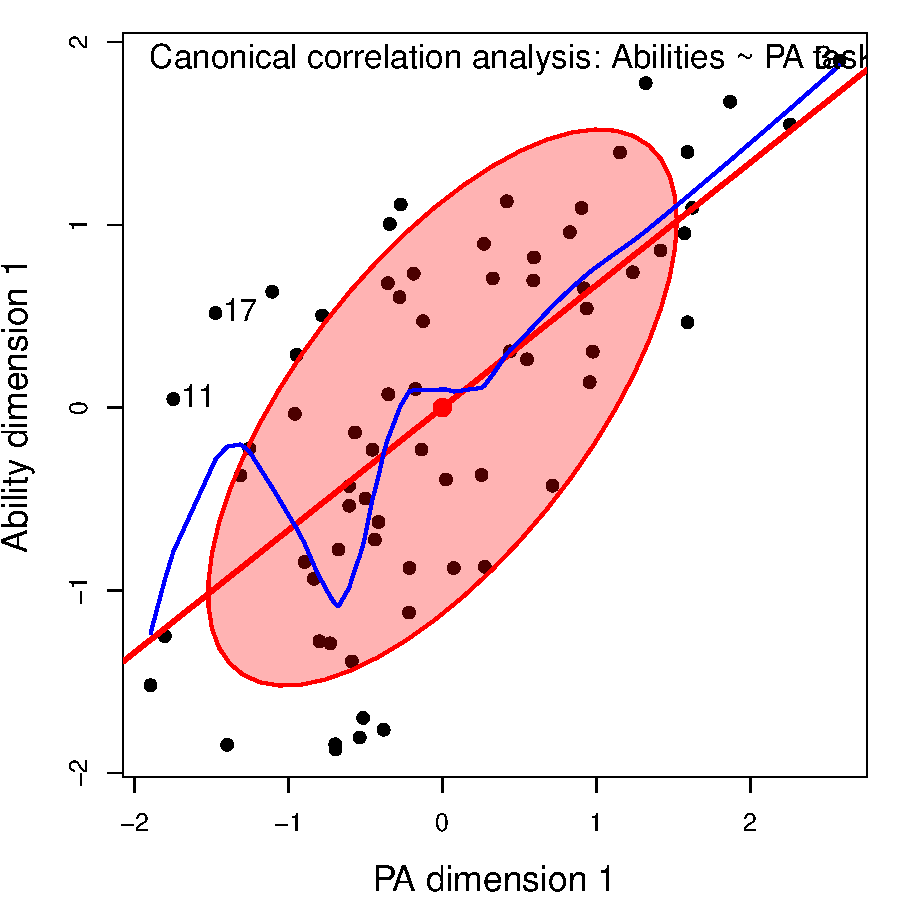
\includegraphics[width=1\linewidth,clip]{figures/rohwer-cancor}
   \end{minipage}%
  \hfill
  \begin{minipage}[c]{.35\textwidth}
   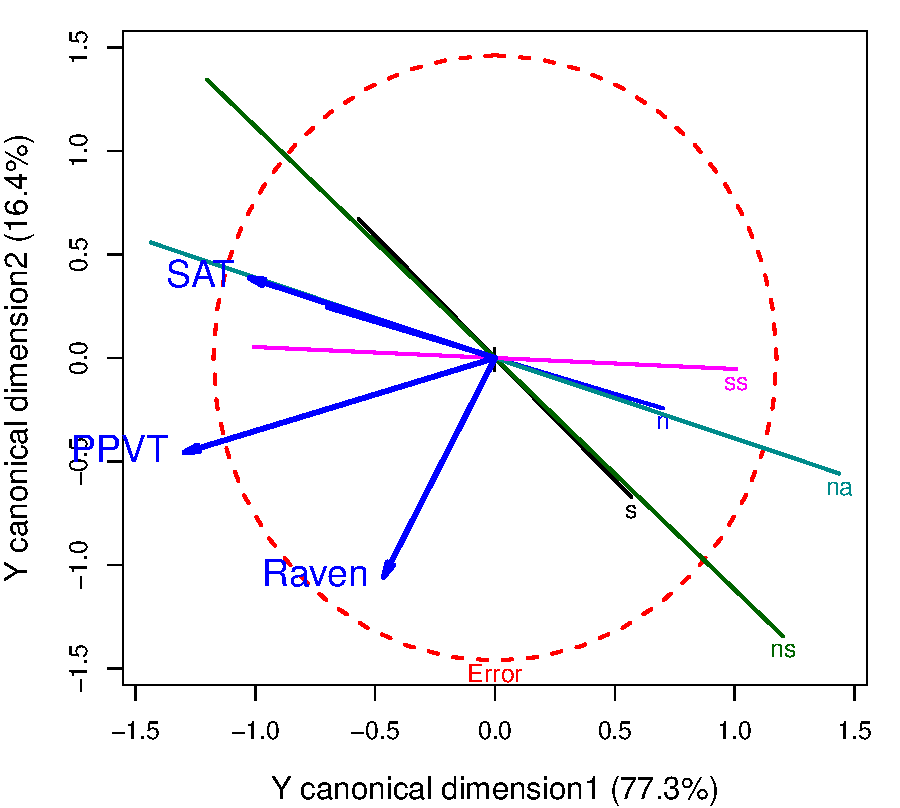
\includegraphics[width=1\linewidth,clip]{figures/rohwer-cancor-HE}
  \end{minipage}
  \hfill
\end{frame}

